\section{Related Work}\label{section:related_work}

\subsection{3-trees}

Following the recursive definition of $k$-trees, 3-trees start with a $K_4$ and every new added vertex is connected to three adjacent vertices. 3-trees inherit a treewidth of 3 and $R$ nodes in the respective $SPQR$ tree since they are triconnected. The box drawing algorithm \ref{al:draw_SPQR} does not suffice for this class of planar graphs since the algorithm does not handle the $R$ node case. Still, it is of interest how the idea of a layered box drawing approach will work out based on the tree decomposition of a 3-tree.

\begin{definition}
	Let $G$ be a 3-tree with its tree decomposition $(T,W)$. $G$ is called \emph{complete}, if the following property holds:
	\begin{itemize}
		\item Every vertex of $T$ is either a leaf or of degree 4
		\item The leaves of $T$ have uniform heights
	\end{itemize}
	In other words, $G$ is called complete if the root of $T$ is the parent of 4 complete tertiary trees of the same height.
\end{definition}

\begin{observation}
	Let $G$ be a complete 3-tree. Applying a layering scheme similar to algorithm \ref{al:complete_outerplanar}, the resulting box drawing $\mathcal{B}_G$ is at least in area bound $\mathcal{O}(n^2)$, when the minimal distance between layers is set to a constant.
\end{observation}

In order validate this observation, a box drawing of $K_4$ is created as illustrated. $K_4$ represents the root of the tree decomposition of a complete 3-tree $G$ with height 0 in its tree decomposition $T$. Let $\mathcal{L}_0$ be the list of layers consisting of the topmost and bottommost layer of the $K_4$ for $h=0$.

\begin{figure}[H]
	\centering
	\begin{subfigure}{\textwidth}
		\centering
		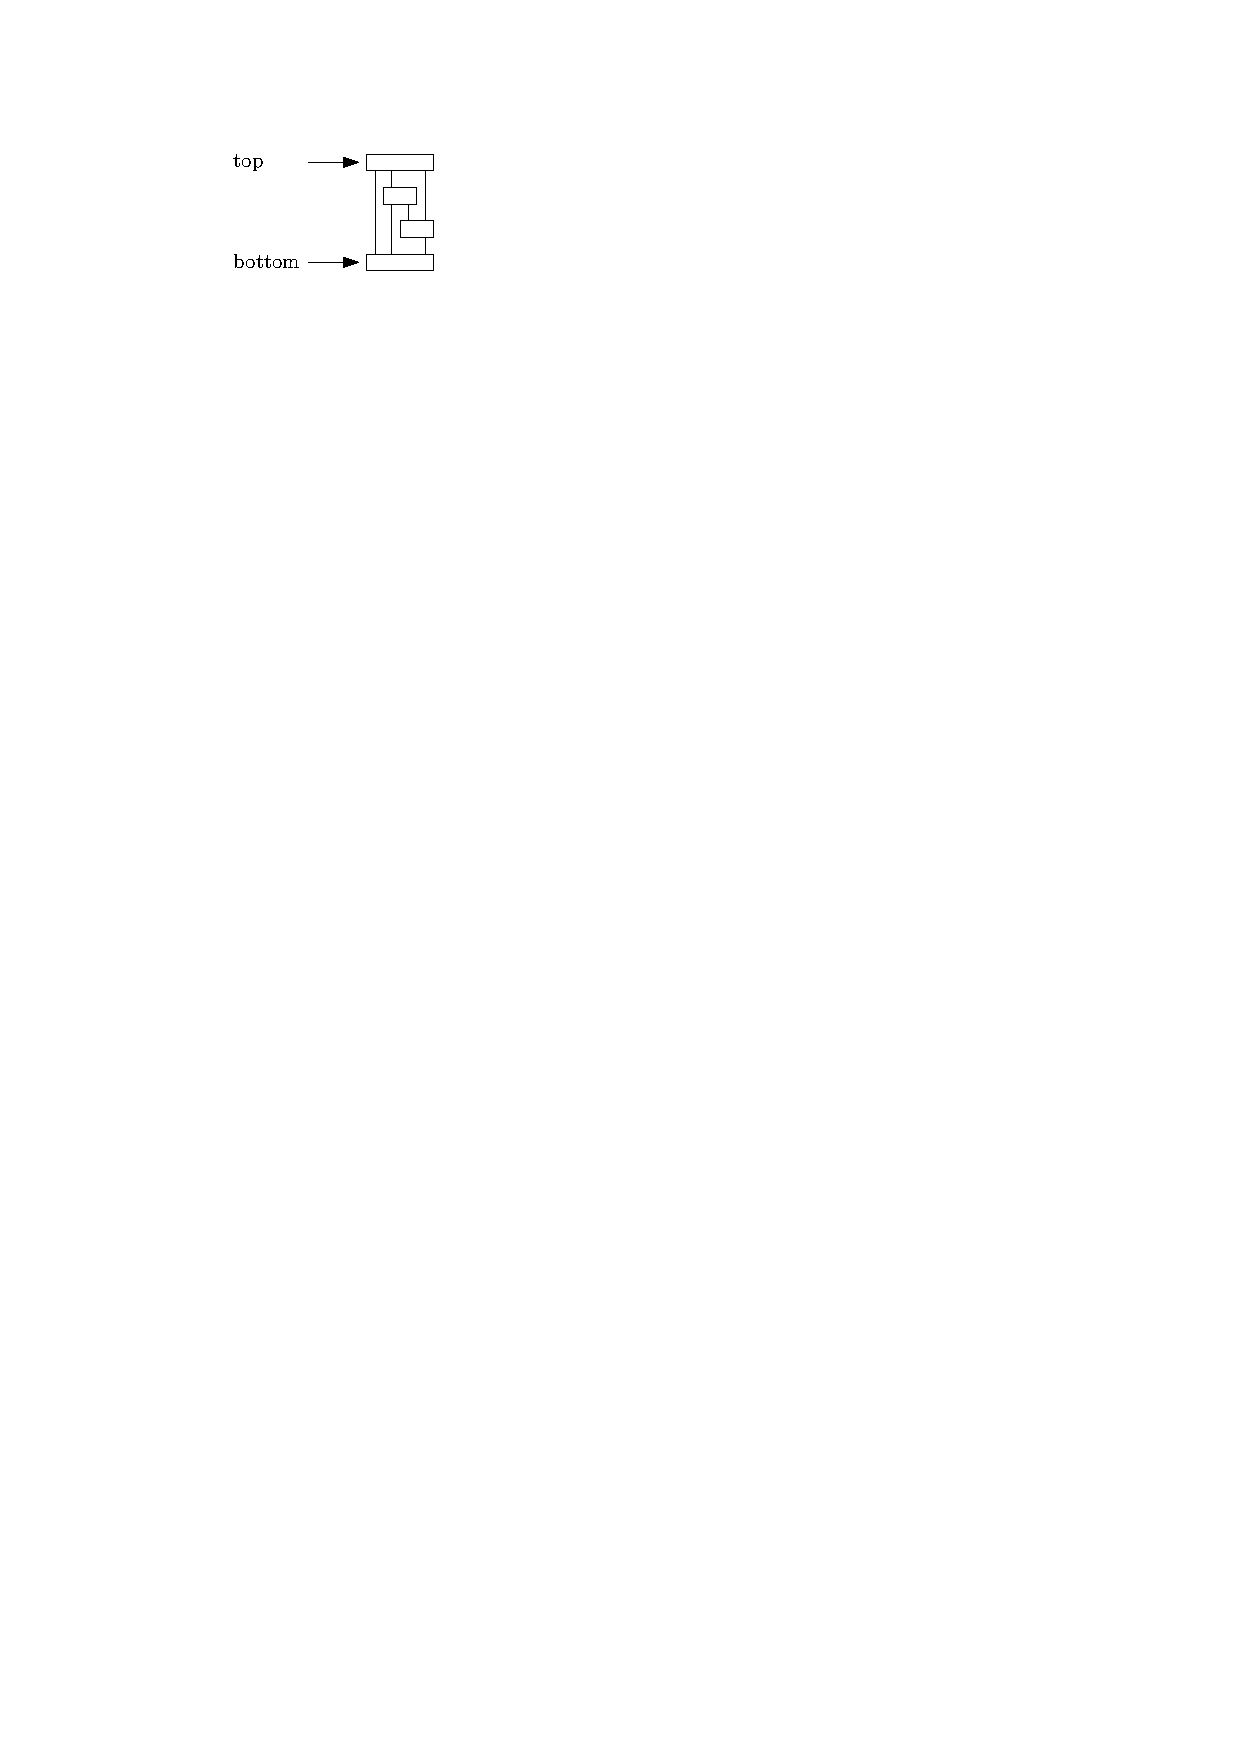
\includegraphics[page=1,width=0.4\linewidth]{graphics/3-tree_example.pdf}
	\end{subfigure}
	\caption*{$K_4$ drawn on four different layers. $\mathcal{L}_0 = (top, bottom)$}
\end{figure}

The amount of layers created while inserting vertices will determine the height of the resulting drawing.  A complete 3-tree $G$ with height $h$ in $T$ is extended to a complete 3-tree $G^+$ with height $h+1$ when for every inner face $f$ a vertex is inserted and connected to the vertices defining $f$. These newly created layers are inserted into $\mathcal{L}_h$ according to their position from top to bottom, resulting in $\mathcal{L}_{h+1}$

\begin{figure}[H]
	\centering
	\begin{subfigure}{\textwidth}
		\centering
		\includegraphics[page=2,width=0.6\linewidth]{graphics/3-tree_example.pdf}
	\end{subfigure}
	\caption*{One layer insertion in $\mathcal{B}$ when extending the height of $T$ from 0 to 1.}
\end{figure}
Let $l$ be the layer where the new vertices are inserted in according to this scheme. Every vertex insertion creates three new faces out of a pre-existing one. Unfortunately, for any layer $l$, there will be a face encapsulated between $l$ and both its predecessor and successor in $\mathcal{L}$.
\begin{figure}[H]
	\centering
	\begin{subfigure}{\textwidth}
		\centering
		\includegraphics[page=3,width=0.6\linewidth]{graphics/3-tree_example.pdf}
	\end{subfigure}
	\caption*{$\mathcal{L} = (top, l, bottom)$}
\end{figure}
So, in order to insert vertices in all the inner faces so that $G$ is a complete 3-tree and the height of $T$ will be incremented by 1, there are $|\mathcal{L}_h|-1$ at least new layers necessary.\\
For a complete 3-tree with height $h$ in its tree decomposition, the total amount of layer insertions is calculated the following way:
\begin{align*}
	&\sum_{i=0}^{h} 2^i = 2^{h+1}-1 \underbrace{\in}_{h\in \mathcal{O}(\log n)} \mathcal{O}(n)
\end{align*}
The resulting box drawing will therefore consume at least $\mathcal{O}(n^2)$ area, when the minimal distance between two layers values a constant. In conclusion, no ratio optimization is possible with this layering approach.